Чтобы продемонстрировать пьзоэффект в кристалле, давайте встанем в произвольную точку
на кривой дифракционного отражения, другими словами выведем интенсивность детектора
из максимума отражения в точку на склоне кривой (Рис.~\ref{ris:kdopiez}).

\begin{figure}[H]
\centering
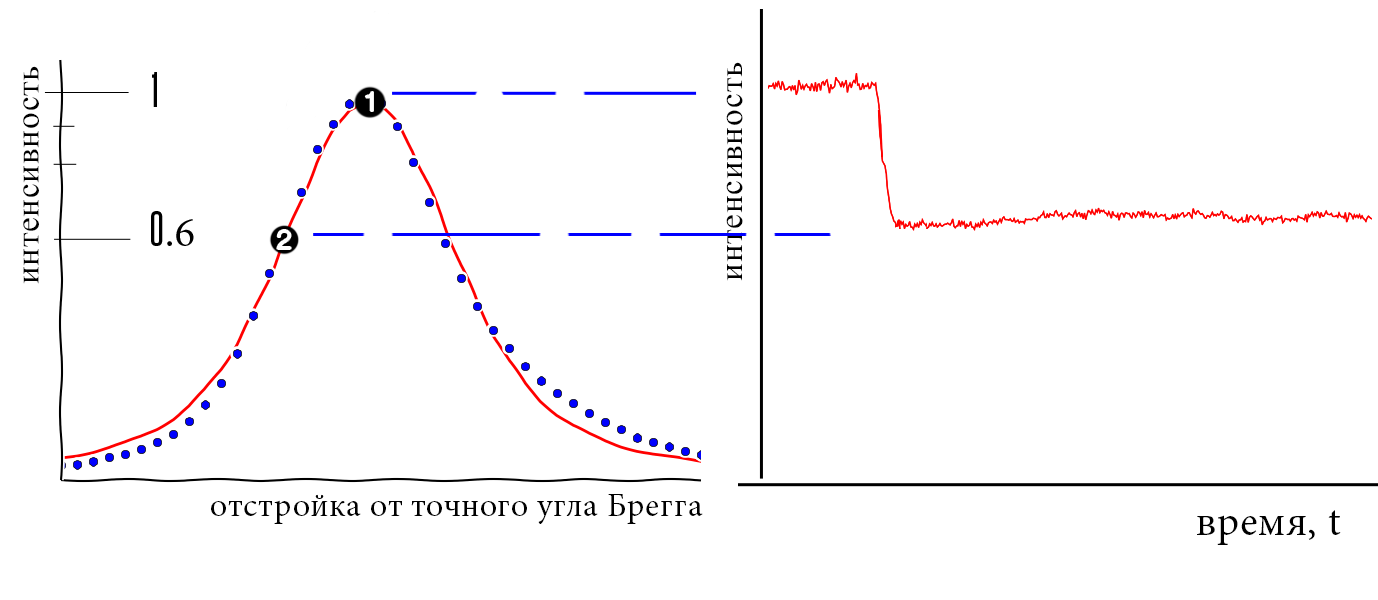
\includegraphics[width=1\linewidth]{images/kdopiez.eps}
\caption{Выбор точки на КДО(справа), интенсивность сигнала детектора(слева)}
\label{ris:kdopiez}
\end{figure}

\par
Теперь включим электрическое поле поочередно в разных направлениях (Рис.~\ref{ris:princip}B).
\par
Наблюдаем смещение кривой (Рис.~\ref{ris:princip}C), т.е.
 прямое изменение интенсивности на детекторе (Рис.~\ref{ris:princip}A).

\begin{figure}[H]
\centering
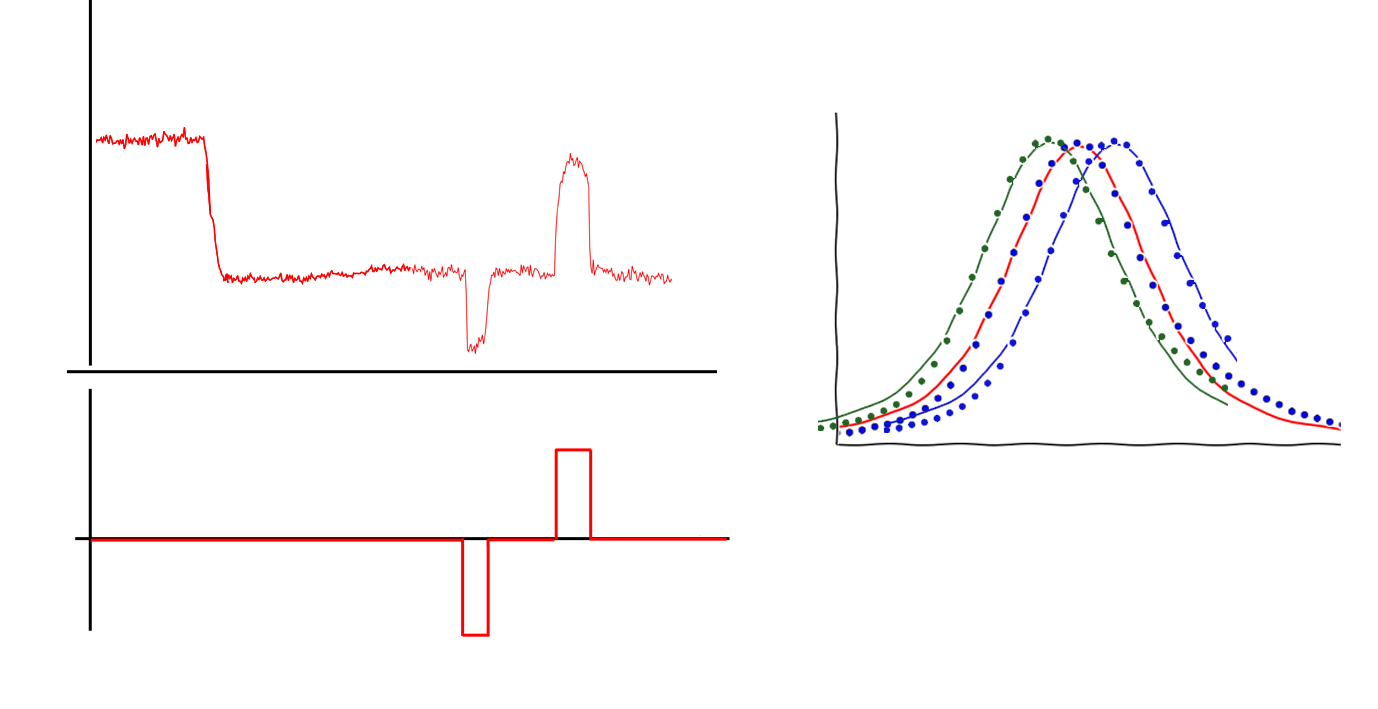
\includegraphics[width=0.8\linewidth]{images/princip.eps}
\caption{A) Интенсивность детектора; В) Разность потенциалов на
поверхности кристалла; С) Положение КДО}
\label{ris:princip}
\end{figure}

\textcolor{mygreen}{
Таким образом представлется возможным отследить перемещение выбранного количества
 точек на КДО в момент подачи поля на кристал. Это позволит нам оценить искомый
 модуль (d33) обратного пьезоэффекта. Исключить ``паразитные'' вклады в смещение кривой
  и сократить ошибку. Так например кристал LBO имеет коэффициент теплового расширения
   в 7 раз превышающий величину для кристаллов кварца и кремния (2:14), ниже будет
   показано влияние температуры на отражение. К тому же, наблюдается уширение кривой,
   а так же смещения в связи с неизвестными нам эффектами, но к нашему везению, время
   действия пьезоэффекта на порядок меньше времени тех процессов которые были перечислены
    (покажем это ниже). Подробный список наблюдений, оказывающих ряд трудностей для измерения -
    приведен в приложении А. Избежать дополнительных эффектов удалось, проводя разовые эксперименты,
    с промежуточными перерывами в 1 час.
}

% \hrulefill \\
